\chapter{Introduction}
%\epigraph{To be sure, a writer cannot begin with a thesis; he must rather use his writerly sensitivity to intuit what is going on, even if he cannot understand its implications.}{--- Gary Morson, \textit{How the great truth dawned}}
\epigraph{If you do not know where you come from, then you don't know where you are, and if you don't know where you are, then you don't know where you're going. And if you don't know where you're going, you're probably going wrong.}{Terry Pratchett}
 
%Gary Saul Morson, How the great truth dawned
%https://www.newcriterion.com/issues/2019/9/how-the-great-truth-dawned

%Taken from https://en.wikipedia.org/wiki/R.U.R.
\section{Autonomy and humanity through the ages}
\begin{wrapfigure}{r}{0.5\textwidth}
  \begin{center}
  	\vspace{-20pt}
    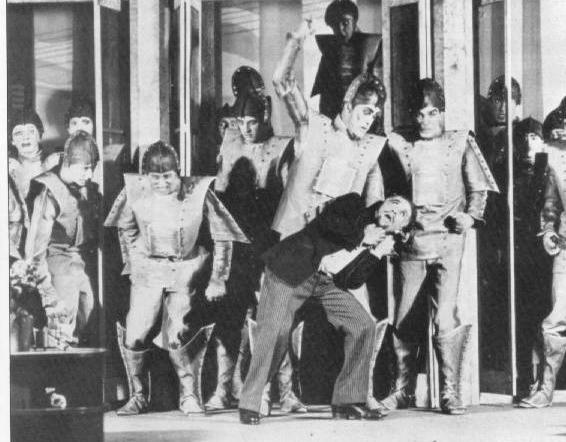
\includegraphics[width=0.4\textwidth]{introduction/rur.jpg}
     \vspace{-15pt}
  \end{center}
  \caption{A robot rebellion from Karel Capek's 1920 play, \textit{Rossum's Universal Robots}.}
  \vspace{-5pt}
  \label{fig:into_rur}
\end{wrapfigure}

This thesis deals with the improvement of autonomous systems, which, in some form or another, have been imagined and realized for the bulk of recorded history. In Greek mythology, the god Hephaestus was said to create talking mechanical hand-maidens, while early Hindu and Buddhist texts tell of \textit{yantakara} that lived in Greece and created machines that helped in trade and farming. The secret methods of the \textit{yantakara} (the early `roboticists') were closely guarded, and mechanical assassins were said to pursue and kill any person who revealed their techniques\footnote{Please be careful distributing this thesis.}. 

%https://scroll.in/article/916490/in-an-ancient-indian-legend-robots-guarded-buddhas-relics
%Cite 


Since the industrial revolution, the idea of an autonomous machine--one that requires no, or very minimal, human intervention or oversight to operate--has been imagined in different ways. Depending on one's perspective, autonomous machines have perennially promised to either usher in a utopia of freedom, or threatened to bring about an age of job loss and social upheaval that worsens socioeconomic divisions. Much like the Luddites of the 19th century, the social critics of the 21st century have continued the dialectic to understand the social ramifications of modern \textit{yantakara} and their newly-created autonomous hand-maidens.

These controversial origins are embedded even within the modern name of for the academic field, \textit{robotics}. The word \textit{robot} comes from an anglicized title of a science fiction play, Rossum's Universal Robots, written by the Czech playwright Karel Capek in 1920 (see \Cref{fig:into_rur}). In naming the play, the word \textit{robot} was derived from the Slavic term for slave, \textit{rab}, and its Czech derivative for serf labour, \textit{rabota}, while the name \textit{Rossum} was inspired by the Czech word for reason, or intellect. Indeed, the concept of enslaved or embodied  intelligence is at the heart of modern definitions of the discipline of robotics \citep{Redfield2019-pi}. Much of the popular culture surrounding robots (e.g., Shelley's \textit{Frankenstein}, Asimov's \textit{I, Robot}, Kubrick's and Clarke's \textit{2001: A Space Odyssey}) also paints a complicated picture of humanity's relationship with such enslaved machines. In this thesis, I focus on improving a specific part of a modern \textit{mobile} autonomy pipeline, while minimizing the use of term \textit{robot} to avoid maelstrom of philosophical and ethical problems that it connotes. I hope my work aids the march of technological progress towards a future which finds some Hegelian synthesis of autonomy and humanity---a future in which human-in-the-loop autonomous systems augment and improve the lot of many people while still negotiating and constantly considering the social costs that come with technological innovation.

\section{Mobile Autonomy and State Estimation}
While the looms and railroads of the industrial revolution were spurred by the discovery of steam engines and electricity, modern \textit{mobile} autonomy was largely born out of the technological arms race of the cold war and the constraints and challenges associated with long-distance flight and extraterrestrial travel (see \cite{Grewal2010-ts} for a history of one of the seminal algorithms in mobile autonomy, the Kalman filter). Indeed, much of the work on modern perception algorithms has its origins in the automated compilation of cold-war-era reconnaissance imagery and the design of extraterrestrial rovers like the Mars Exploration Rovers, \textit{Spirit} and \textit{Opportunity} \citep{Scaramuzza2011-qr}. Much of the planning and control algorithms originate in American and Soviet defence-funded research \citep{Nilsson1984-oc,Thrun2006-hb}.

%https://mars.nasa.gov/resources/22342/opportunity-legacy-pan-true-color/
\begin{figure}
  \begin{center}
  	\vspace{-10pt}
    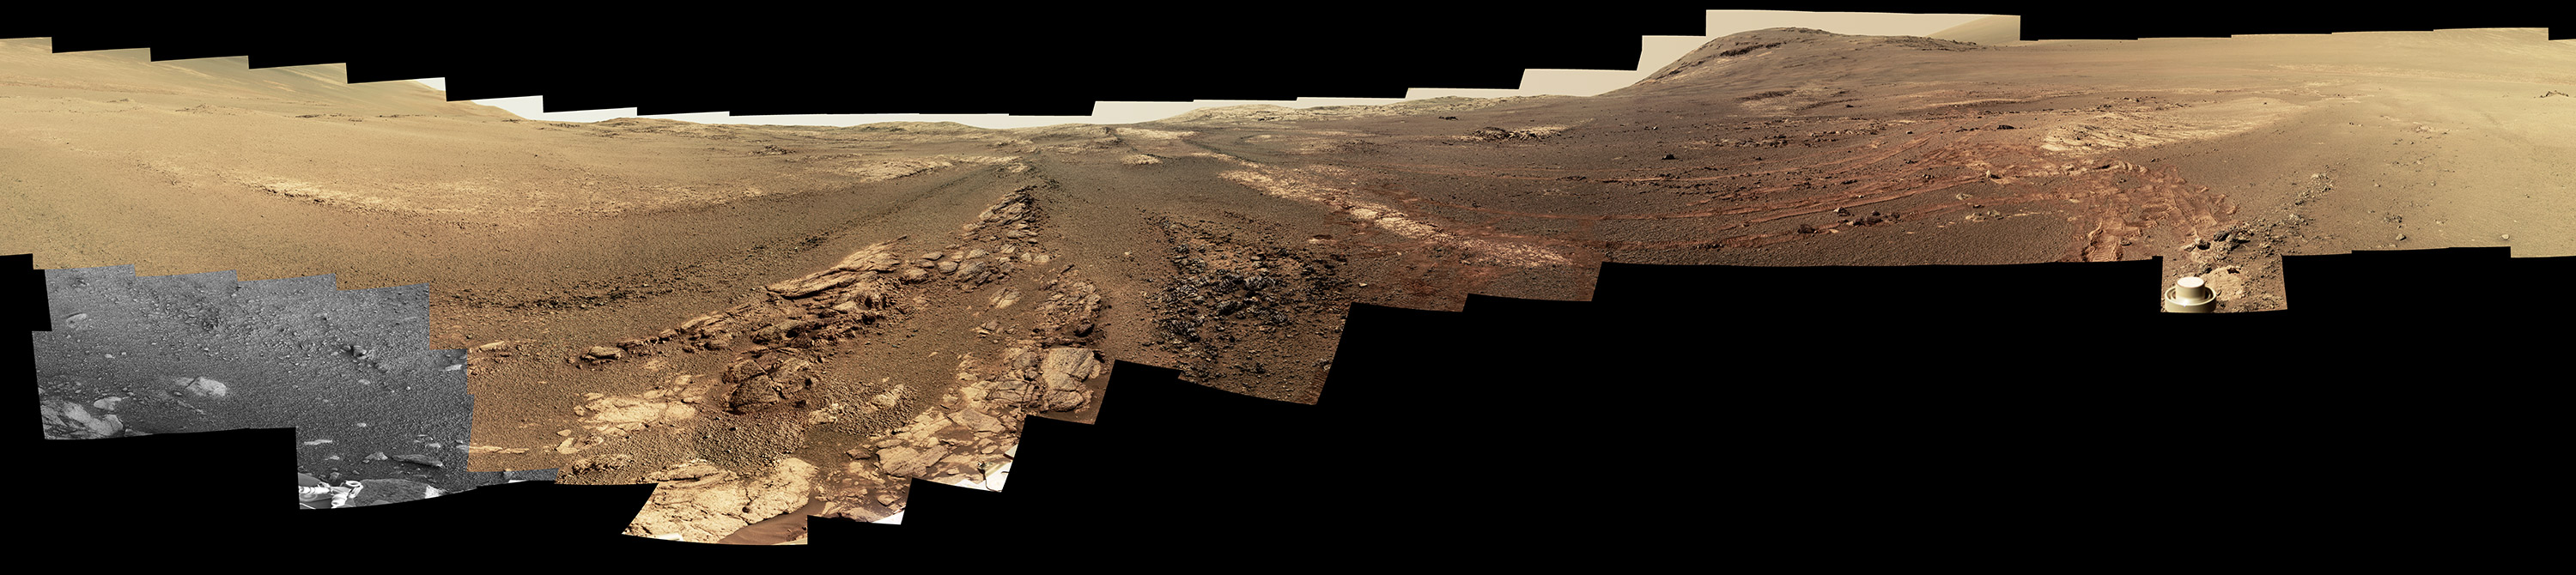
\includegraphics[width=0.95\textwidth]{introduction/pancam-panorama-opportunity}
     \vspace{-15pt}
  \end{center}
  \caption{The last 360 degree panorama taken by the PanCam apparatus of the Mars Exploration Rover, \textit{Opportunity}, at its final resting place on Mars, the western rim of the Endeavour Crater. Contact with \textit{Opportunity} was lost shortly after this was captured, due to a severe dust storm. (Credit: NASA/JPL-Caltech/Cornell/ASU).}
  \vspace{-5pt}
  \label{fig:into_rur}
\end{figure}


Once confined to carefully-controlled factories, autonomous mobile platforms have now began to show great promise in improving the safety of human transport, reducing the burden of repetitive, arduous jobs, and more efficiently leveraging limited resources for environmental monitoring. This newly-realized potential can be attributed to several factors: improvements in the cost and efficiency of computing devices (in terms energy efficiency, processing power, and overall size), the availability of relatively cheap, compact, high-quality sensors and rapid prototyping tools, and the development of open-source hardware, software platforms and datasets (e.g., the Robot Operating System, the KITTI Self-Driving Car dataset \citep{Geiger2013-ky}). 

 
 Despite decades of research, mobile autonomy as a field still has nebulous demarcations between subfields. I have attempted to provide a general overview of the field through a series of Venn diagrams in \Cref{fig:intro_three_venn}.  At the highest level, the field can be roughly divided into those researchers who study and develop software, those who study and develop hardware, and those who study and analyze the interaction between autonomous systems (composed of both software and hardware) and humans (\Cref{fig:intro_autonomy_venn}). There is, of course, a plethora of overlap between all three of these rough categories. Within the software realm, there has historically been a distinction between those who study algorithms that deal with the perception of the interoceptive and exteroceptive data, those who study how to use that data to plan action, and those who study how to use those plans to control a system to execute that action (\Cref{fig:intro_software_venn}). 
 
 %Add some discussion about computer science vs. robotics research
 
 Within perception, which is the focus of this thesis, there are three general directions of research: localization, mapping and object detection and tracking. Localization and mapping can refer to self-localization, or egomotion estimation, which deals with the problem of estimating the pose of a moving platform through an unknown world, SLAM, simultaneous localization and mapping, which deals with the former problem and mapping simultaneously and finally, it can refer to localization within a known map given some hitherto unseen observation of that environment. The field of object detection and tracking (whether that be static objects like stop signs, or moving objects like humans, animals or vehicles) uses much of the same underlying mathematics as the former two, but has historically been a separate strand of research. Broadly, the overlap of all three of these pursuits within the field of autonomy and robotics is referred to as \textit{state estimation} \cite{Barfoot2017-ri}.  
 %https://tex.stackexchange.com/questions/9681/how-to-draw-venn-diagrams-especially-complements-in-latex 
\begin{figure}
     \centering
     \begin{subfigure}[b]{0.3\textwidth}
         \centering
\def\firstcircle{(0,0) circle (2cm)}
\def\secondcircle{(60:2.75cm) circle (2cm)}
\def\thirdcircle{(0:2.75cm) circle (2cm)}
\scalebox{0.75}{
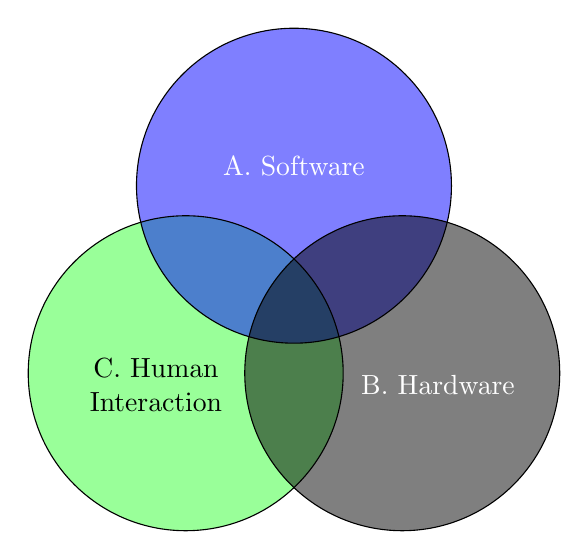
\begin{tikzpicture}
    \begin{scope}[shift={(3cm,-5cm)}, fill]
        \fill[green!80,opacity=0.5] \firstcircle;
        \fill[blue,opacity=0.5] \secondcircle;
        \fill[black,opacity=0.5] \thirdcircle;
        \draw \firstcircle node [yshift=-1ex,xshift=-2.5ex,align=center] {C. Human\\Interaction};
        \draw \secondcircle node [above,color=white] {A. Software};
        \draw \thirdcircle node [yshift=-1ex,xshift=3ex,color=white] {B. Hardware};
    \end{scope}
\end{tikzpicture}         
}
\caption{Research strands in mobile autonomy.}
 \label{fig:intro_autonomy_venn}
     \end{subfigure}
     \hfill
     \begin{subfigure}[b]{0.3\textwidth}
         \centering
\def\firstcircle{(0,0) circle (2cm)}
\def\secondcircle{(60:2.75cm) circle (2cm)}
\def\thirdcircle{(0:2.75cm) circle (2cm)}
\scalebox{0.75}{
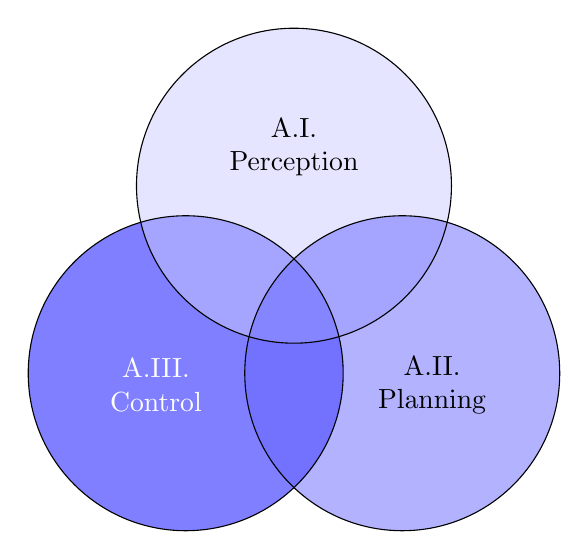
\begin{tikzpicture}
    \begin{scope}[shift={(3cm,-5cm)}, fill]
        \fill[blue,opacity=0.5] \firstcircle;
        \fill[blue!20,opacity=0.5] \secondcircle;
        \fill[blue!60,opacity=0.5] \thirdcircle;
        \draw \firstcircle node [align=center,yshift=-1ex,xshift=-2.5ex,color=white] {A.III.\\Control};
        \draw \secondcircle node [above,align=center,color=black] {A.I.\\Perception};
        \draw \thirdcircle node [align=center,yshift=-1ex,xshift=2.5ex] {A.II.\\ Planning};
    \end{scope}
\end{tikzpicture} 
}        \caption{The components of software research.}
         \label{fig:intro_software_venn}
 \end{subfigure}
 \hfill
      \begin{subfigure}[b]{0.3\textwidth}
         \centering
\def\firstcircle{(0,0) circle (2cm)}
\def\secondcircle{(60:2.75cm) circle (2cm)}
\def\thirdcircle{(0:2.75cm) circle (2cm)}
\scalebox{0.75}{
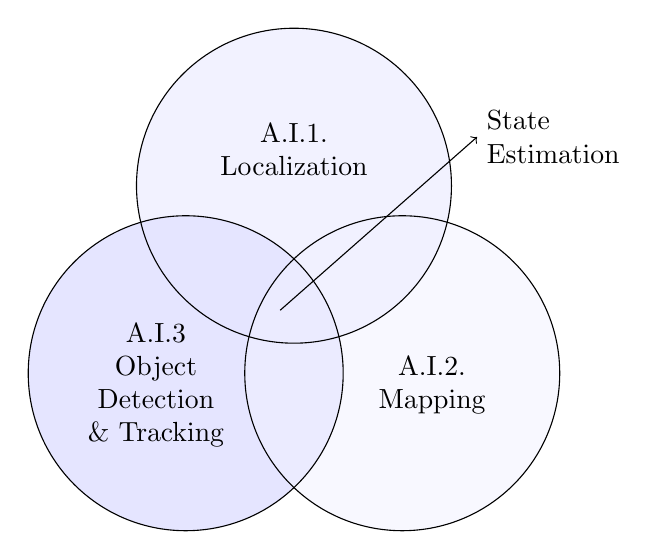
\begin{tikzpicture}
    \begin{scope}[shift={(3cm,-5cm)}, fill]
        \fill[blue!20,opacity=0.5] \firstcircle;
        \fill[blue!10,opacity=0.5] \secondcircle;
        \fill[blue!5,opacity=0.5] \thirdcircle;
        \draw \firstcircle node [align=center,yshift=-1ex,xshift=-2.5ex] {A.I.3\\Object\\Detection\\ \& Tracking};
        \draw \secondcircle node [above,align=center] {A.I.1.\\Localization};
        \draw \thirdcircle node [align=center,yshift=-1ex,xshift=2.5ex] {A.I.2.\\Mapping};
        \draw[->] (1.2,0.8) -- (3.7,3) node[right,align=left] {State\\Estimation};
    \end{scope}
\end{tikzpicture} 
}        \caption{The components of perception.}
         \label{fig:intro_perception_venn}
 \end{subfigure}
        \caption{Venn diagrams of modern mobile autonomy.}
        \label{fig:intro_three_venn}
\end{figure}


\section{The \textit{State} of State Estimation}

\begin{figure}
\begin{center}
		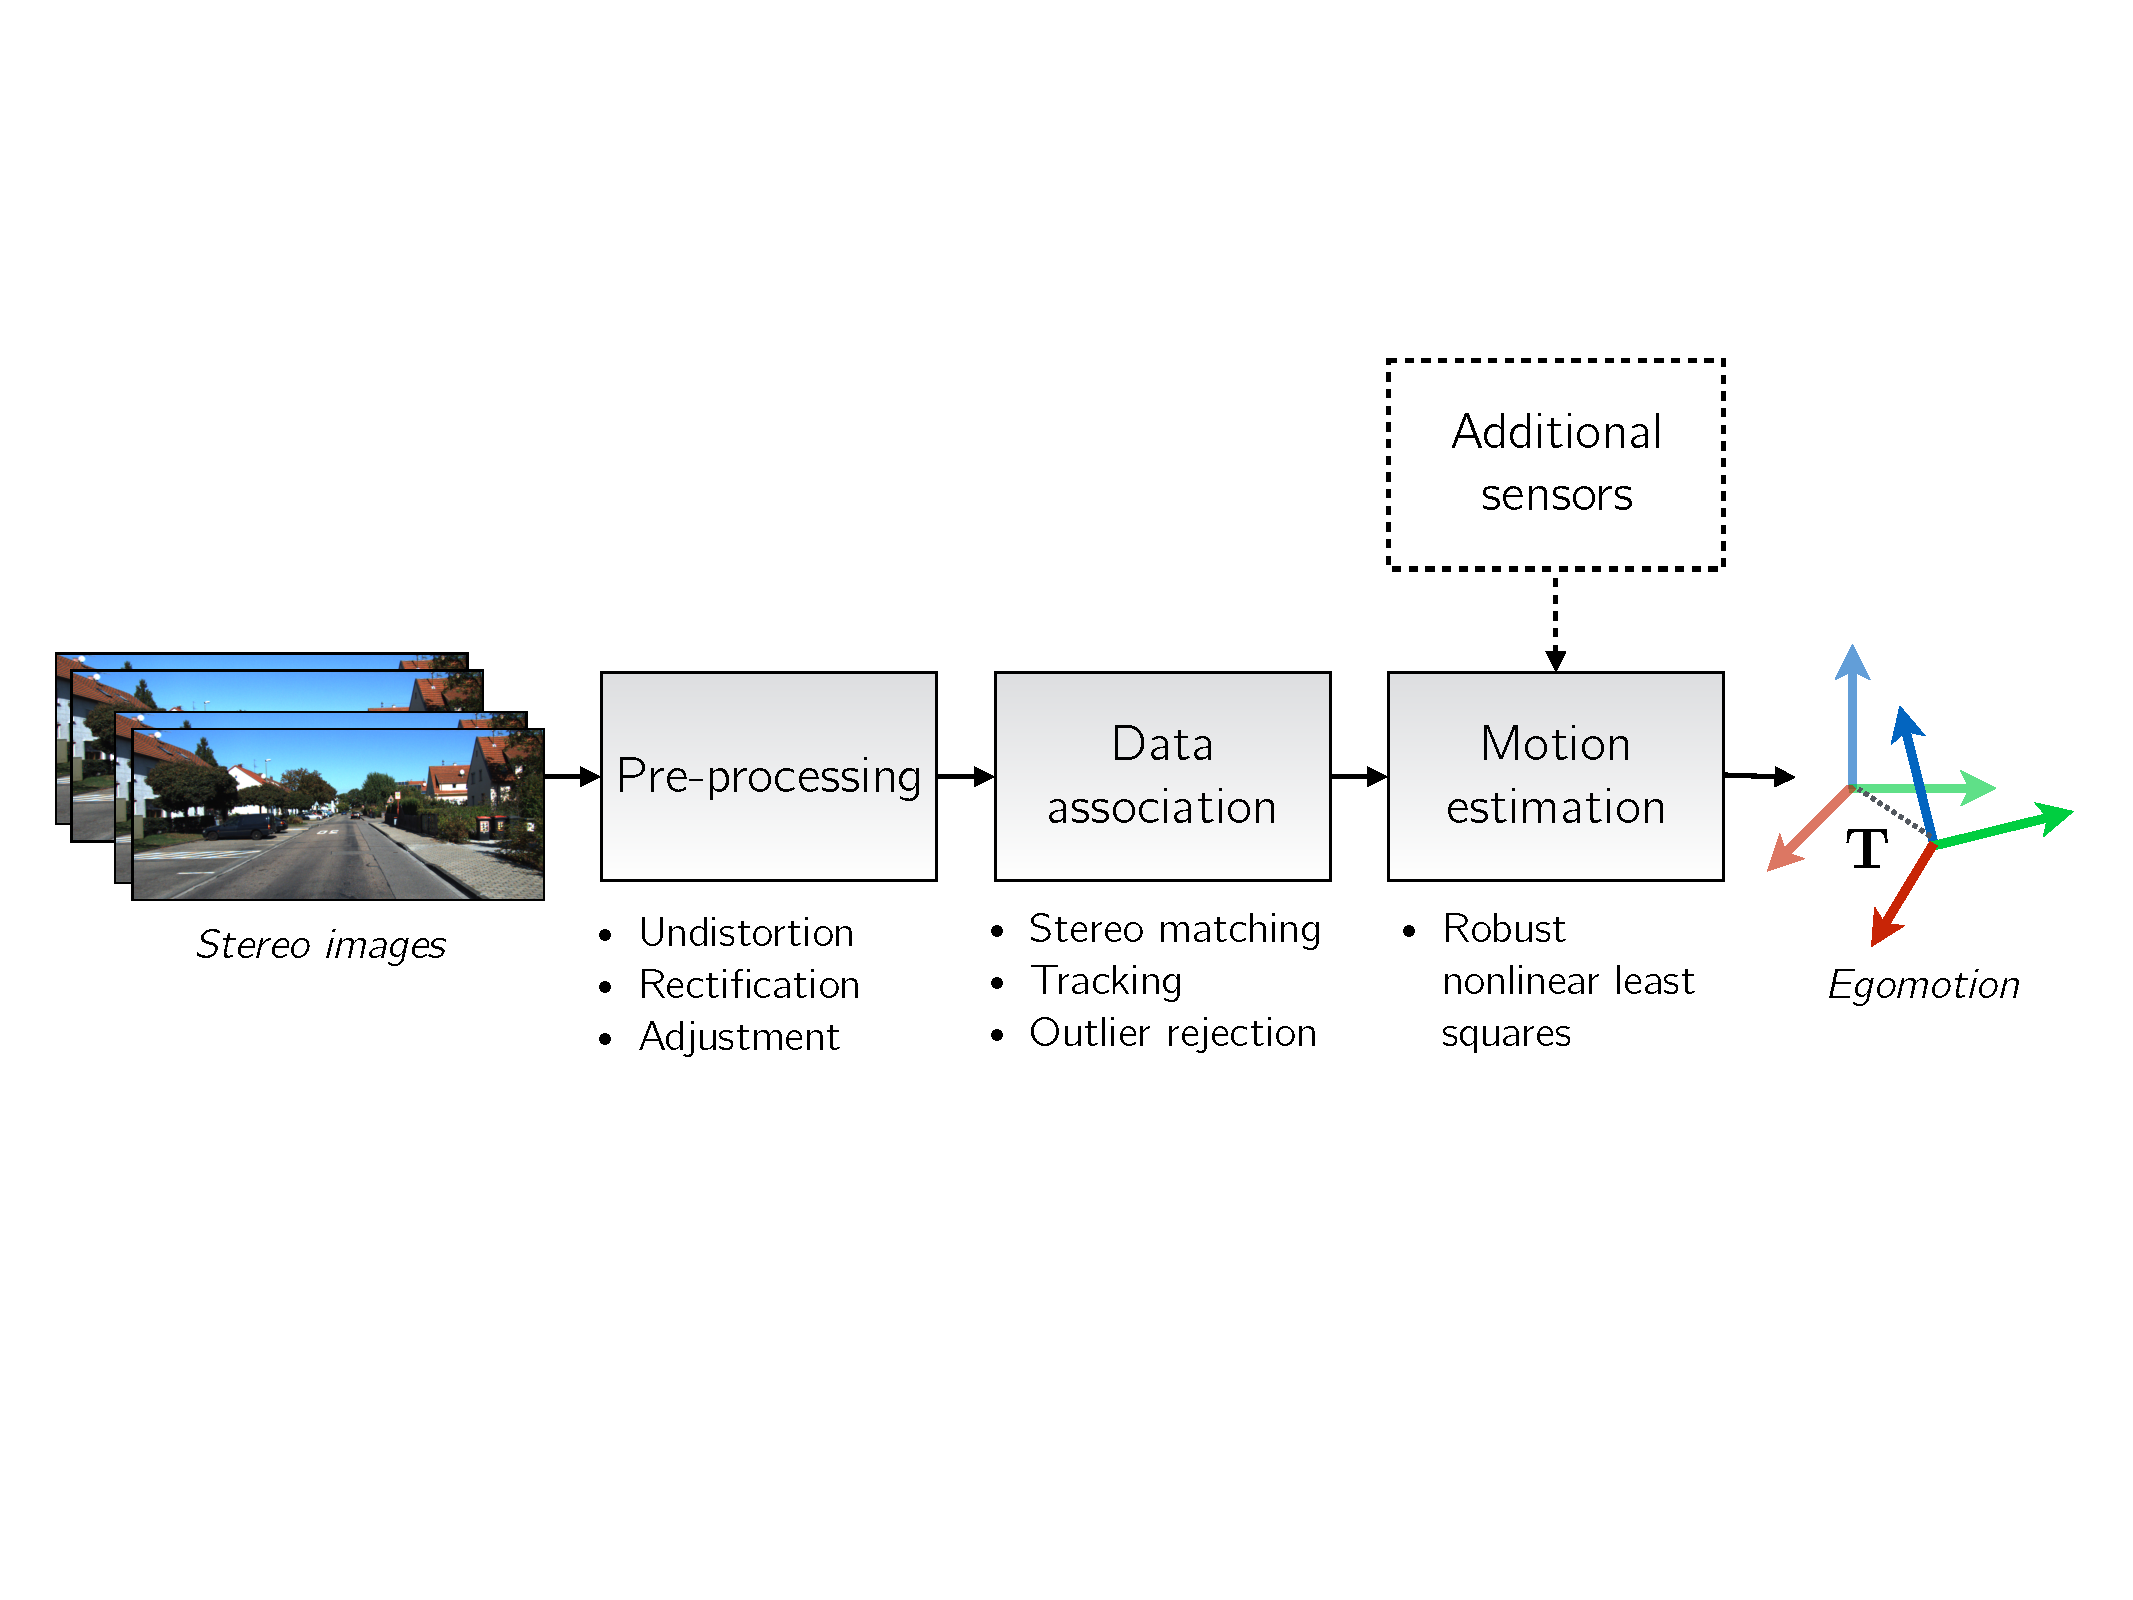
\includegraphics[width=0.98\textwidth]{introduction/vo_pipeline.pdf}
		\caption{A `classical' visual odometry pipeline consists of several distinct components that have interpretable inputs and outputs.}
  	\label{fig:intro_vo_pipeline}
\end{center}
\end{figure}


Central to \textit{classical} state estimation algorithms (which, in this context, refers to the bulk of state estimation research published prior to 2016) is the idea of a pipeline. A pipeline consists several distinguishable blocks that have interpretable inputs and outputs.  By quantifying information contained within sensor data, pipelines facilitate the construction of complex state estimation architectures that can fuse observations from sensors of varied modality to create rich models of the external world and infer the state of a mobile robot within it. My thesis focuses on egomotion estimation: the problem of accurately and consistently estimating the relative pose of a moving robot. For this task, a variety of different sensors may be useful (e.g., lidar, stereo cameras, or inertial measurement units), and each may allow for various components of a state estimation pipeline. For cameras that process visual data, egomotion estimation is referred to as visual odometry or VO and a typical VO pipeline is illustrated in \Cref{fig:intro_vo_pipeline}. 




These types visual egomotion estimation pipelines \citep{Leutenegger2015-fk, Cvisic2015-mt, Tsotsos2015-qs} have achieved impressive localization accuracy on trajectories spanning several kilometres by carefully extracting and tracking sparse visual features (using \textit{hand-crafted} algorithms) across consecutive images. Simultaneously, significant effort has gone to developing localization pipelines that eschew sparse features in favour of  \textit{dense} visual data \citep{Alcantarilla2016-kv, Forster2014-bm}, \todo{Add some modern citations here} typically relying on loss functions that use direct pixel intensities. 


However, in the last several years, a significant part of the state estimation literature has focused on the idea of replacing classical pipelines with parametric modelling through deep convolutional neural networks (CNNs) and data-driven training. Although initially developed for image classification  \citep{LeCun2015-qf}, CNN-based measurement models have been applied to numerous problems in geometric state estimation (e.g., homography estimation \citep{DeTone2016-ue}, single image depth reconstruction \citep{Garg2016-ip},  camera re-localization \citep{Kendall2016-zf}, place recognition \citep{Sunderhauf2015-is}). A number of recent CNN-based approaches have also tackled the problem of egomotion estimation, often purporting to obviate the need for classical visual localization pipelines by learning pose changes \textit{end-to-end}, directly from image data (e.g., \cite{Melekhov2017-dl}, \cite{Handa2016-hm}, \cite{Oliveira2017-lt}).

Despite this surge of excitement, significant debate has emerged within the robotics and computer vision communities regarding the extent to which deep models should replace existing geometric state estimation algorithms. Owing to their representational power, deep models may move the onerous task of selecting `good' (i.e., robust to environmental vagaries and sensor motion) visual features from the roboticist to the learned model. By design, deep models also provide a straight-forward formulation for using \textit{dense} data while being flexible in their loss function, and taking full advantage of modern computing architecture to minimize run time. Despite these potential benefits, current deep regression techniques for state estimation often generalize poorly to new environments, come with few analytical guarantees, and provide only point estimates of latent parameters.

\begin{figure}
\begin{center}
		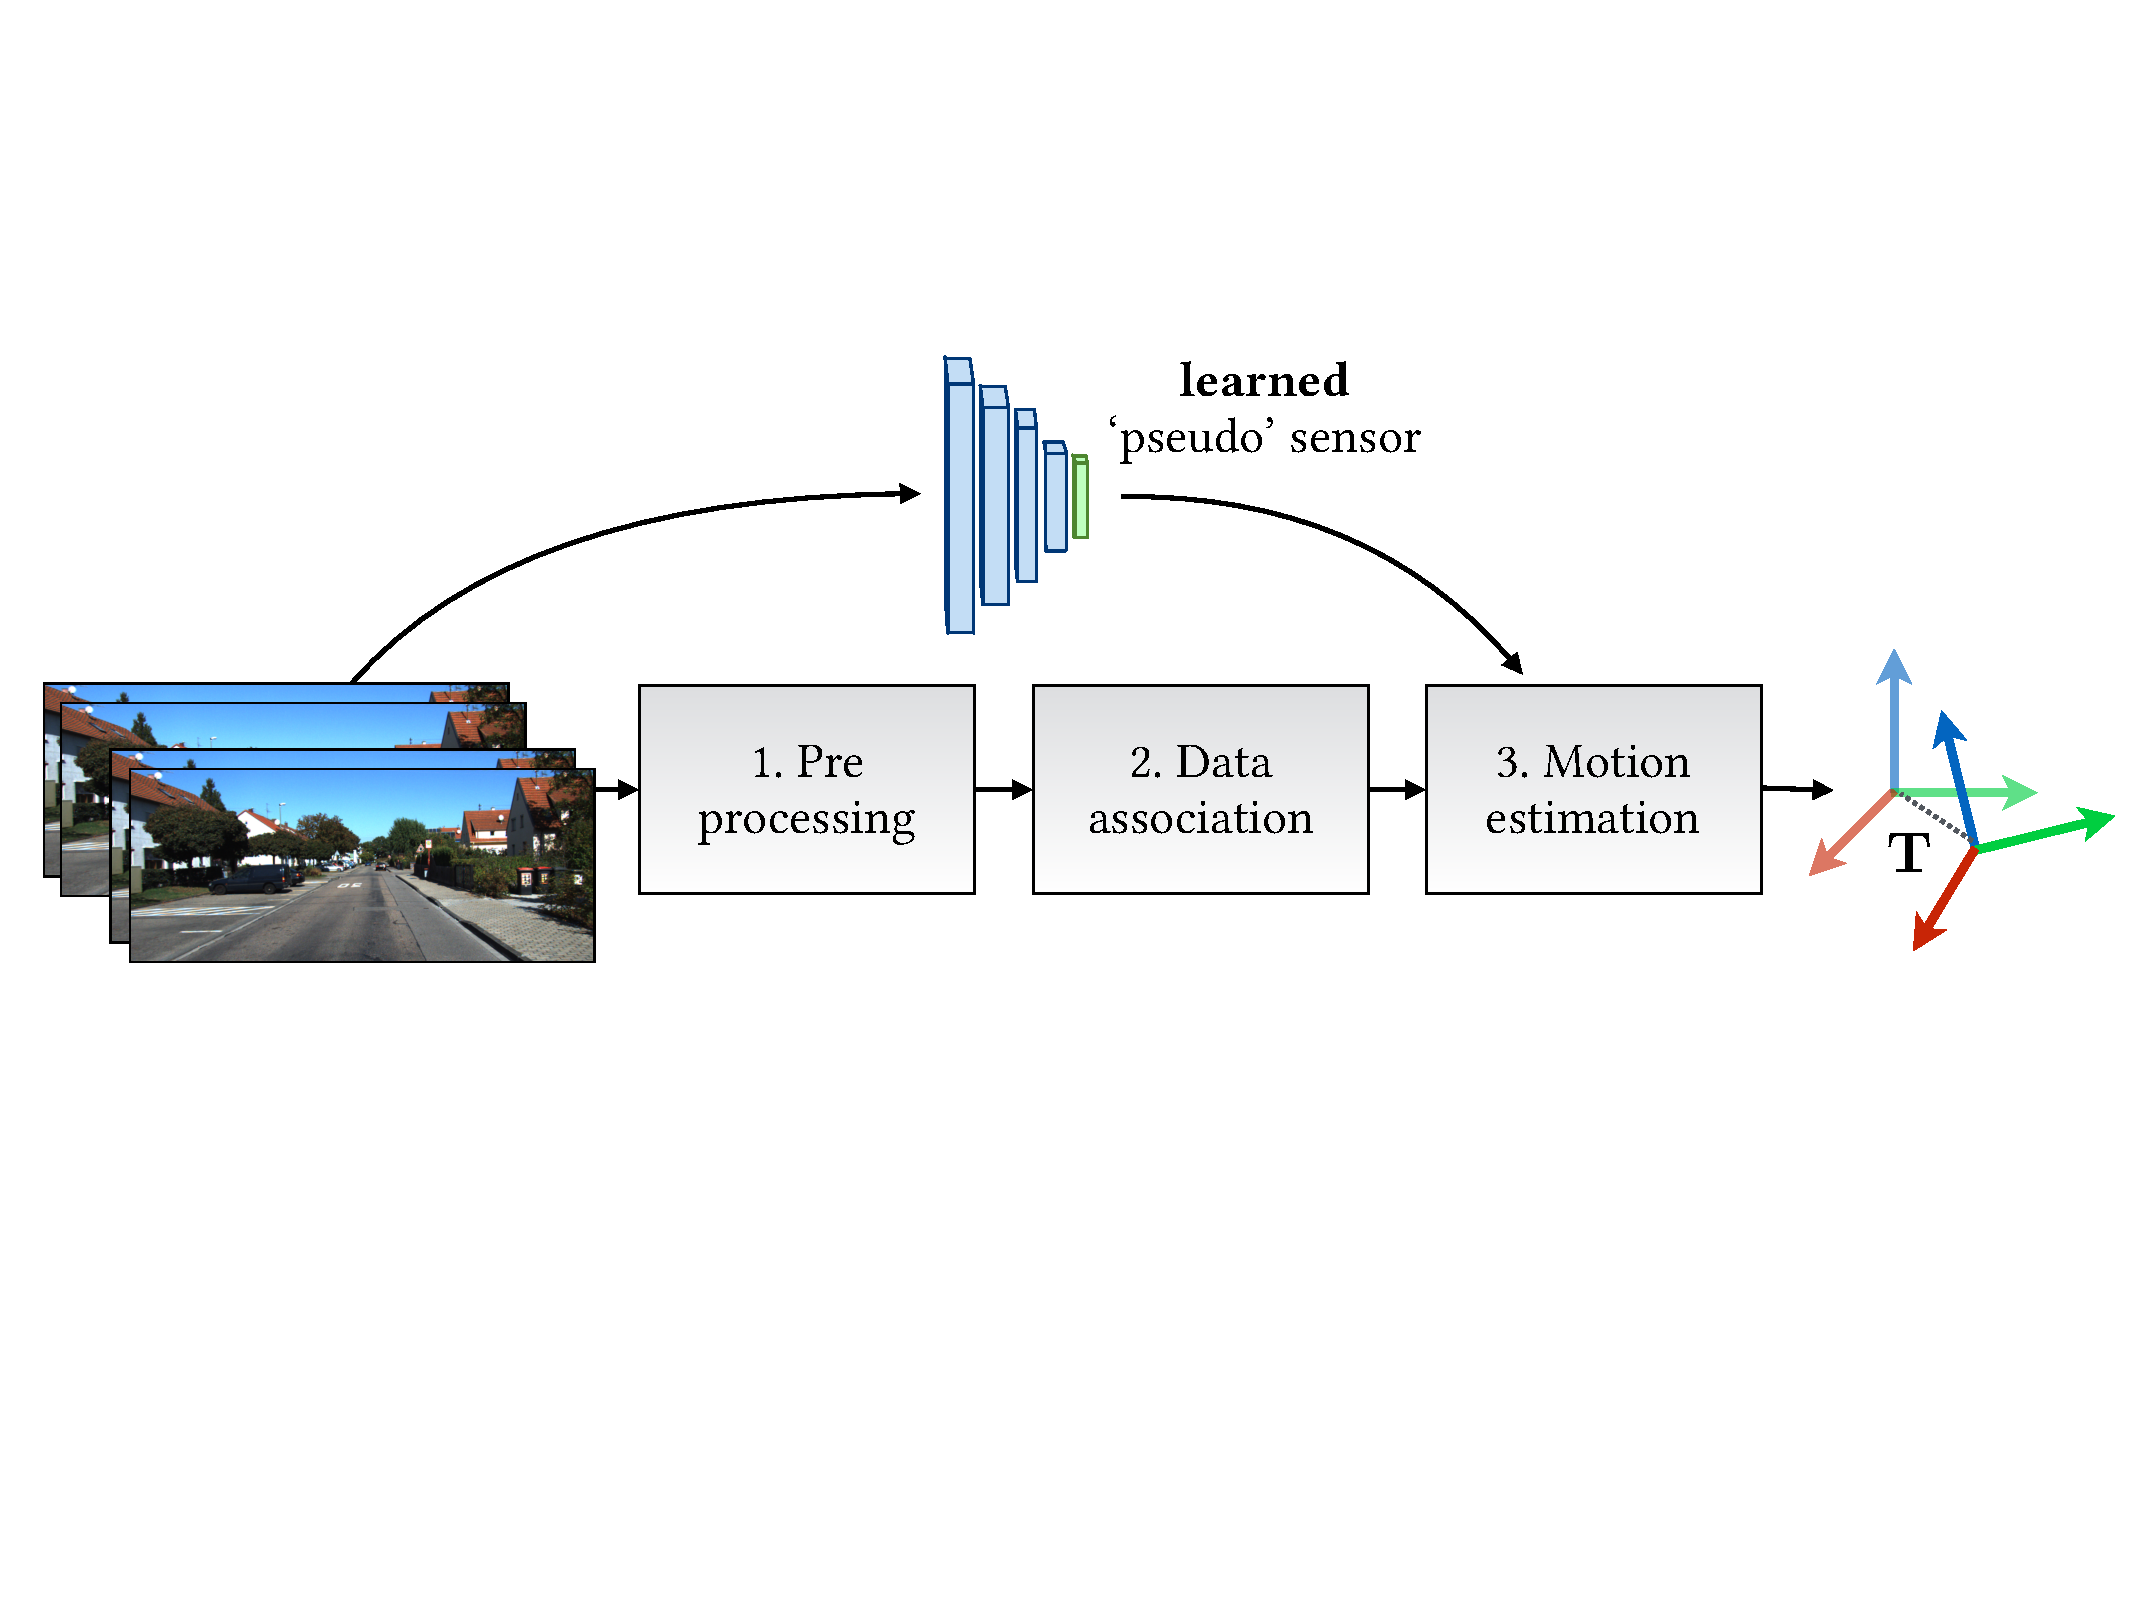
\includegraphics[width=0.98\textwidth]{introduction/pseudo_sensor.pdf}
		\caption{A learned \textit{pseudo-sensor} extracts latent information from the same data stream.}
  	\label{fig:intro_pseudo_sensor}
\end{center}
\end{figure}

\section{Pipelines vs. Parametric Learning}


\begin{table}[h!]
	\caption{The benefits and downsides to using learning.}
	\begin{threeparttable}
	\begin{tabular}{m{0.18\textwidth}m{0.38\textwidth}m{0.38\textwidth}}
		\toprule
		& \textbf{Classical Pipelines} & \textbf{Parametric Learning} \\ \midrule  
		\textit{Maturity} & Decades of literature \& domain knowledge & Nascent in autonomy \\
		& & \\
		\textit{Interpretability} & Good, each component has interpretable input and output & Poor, often with no interpretable intermediate outputs \\
		& & \\
		\textit{Uncertainty} & Foundational to probabilistic robotics & Some methods (bootstrap, BCNNs)  \\
		& & \\
		\textit{Robustness} & Relatively good & Highly dependant on training data\\
		& & \\
		\textit{Flexibility} & Limited by components & Limited by training data \\
		\bottomrule
	\end{tabular}
\end{threeparttable}
\label{tab:7scenes_stats}
\end{table}

There is new evidence that separating different tasks into interpretable components (e.g., optical flow, scene segmentation) works better than end-to-end learning for action \citep{Zhou2019-se}.

\section{The Learned Pseudo-Sensor}

To retain the benefits of classical state estimation pipelines while leveraging the representational power of modern deep parametric networks, I suggest the paradigm of the \textit{learned pseudo-sensor}. Classical pipelines have shown to be relatively robust across numerous types of environments. Instead of completely replacing them, my thesis presents several ways in which machine learning techniques can be used to 

%\section{Outstanding Issues in the Field}

%\subsection{The limits of homoscedastic noise models}
%
%Although several state-of-the-art state estimation pipelines  \citep{Leutenegger2015-fk, Cvisic2015-mt} leave observation uncertainty associated with sensor measurements as a static tuning parameter, recent work \citep{Vega-Brown2014-sb, Hu2015-uw} suggests that using a stationary, homoscedastic noise in observation models can often reduce the consistency and accuracy of state estimates. This is especially true for complex, inferred measurement models. In foot-mounted navigation, the inferred zero velocity detector may be more or less informative depending on the exact type of motion and individual gait. In visual data, inferred visual observations can be degraded not only due to sensor imperfections (e.g. poor intrinsic calibration, digitization effects, motion blur), but also as a result of the observed environment (e.g. self-similar scenes, specular surfaces, textureless environments). Indeed, robust costs \cite{Alcantarilla2016-kv, MacTavish2015-wt, Agarwal2013-jq} and whiteness tests \citep{Tsotsos2015-qs} have commonly been used to alleviate the problem of poor noise modelling, but more work is required to better learn uncertainty in complex measurement models.
%
%
%\subsection{Deep, learned models with no uncertainty estimates}
%
%Although the paradigm of deep neural networks has resulted in several significant achievements in the fields of computer vision \citep{LeCun2015-qf}, these types of models have largely focused on point estimates (in either regression or classification) without any principled uncertainty estimates. Recently, the regularization techniques of dropout and dropconnect in Convolutional Neural Networks have been linked with approximate variational inference in homoscedastic Gaussian Processes \citep{Gal2015-bf, Kendall2016-zf, McClure2016-ai}, and the statistical technique of \textit{bootstrapping} has been applied to Deep Q Networks \citep{Osband2016-jg} to infer uncertainty, but both techniques are in their infancy. Recent work \citep{Osband_undated-wl} has also suggested that the former technique of dropout-based `uncertainty' is actually a measure of \textit{risk} (i.e., stochasticity in the measurements) and not \textit{uncertainty} over state parameters. Further, the same work showed that even this risk quantification can be arbitrarily bad given a fixed dropout parameter (which is typically the case).
%
%\subsection{Integration of deep models into state estimation pipelines}
%
% To integrate the power of deep networks into state estimation algorithms, the recent literature differs in how to proceed. While some attempt to parametrize geometric transformations in their unconstrained state, and then learn the resulting state within a deep network regression optimization \citep{Costante2016-hb, Kendall2015-kh}, others integrate deep networks within outer estimation loops \citep{Haarnoja2016-ph}. Yet other work has used the neural network as an error correcting mechanism on top on an existing kinematic or dynamic model \citep{Punjani2015-pj}. This integration is made more difficult by the lack of uncertainty estimates associated with many learned measurement models in the computer vision and machine learning literature.
% 
 
\section{Original Contributions}

\begin{figure}[h!]
\begin{center}
		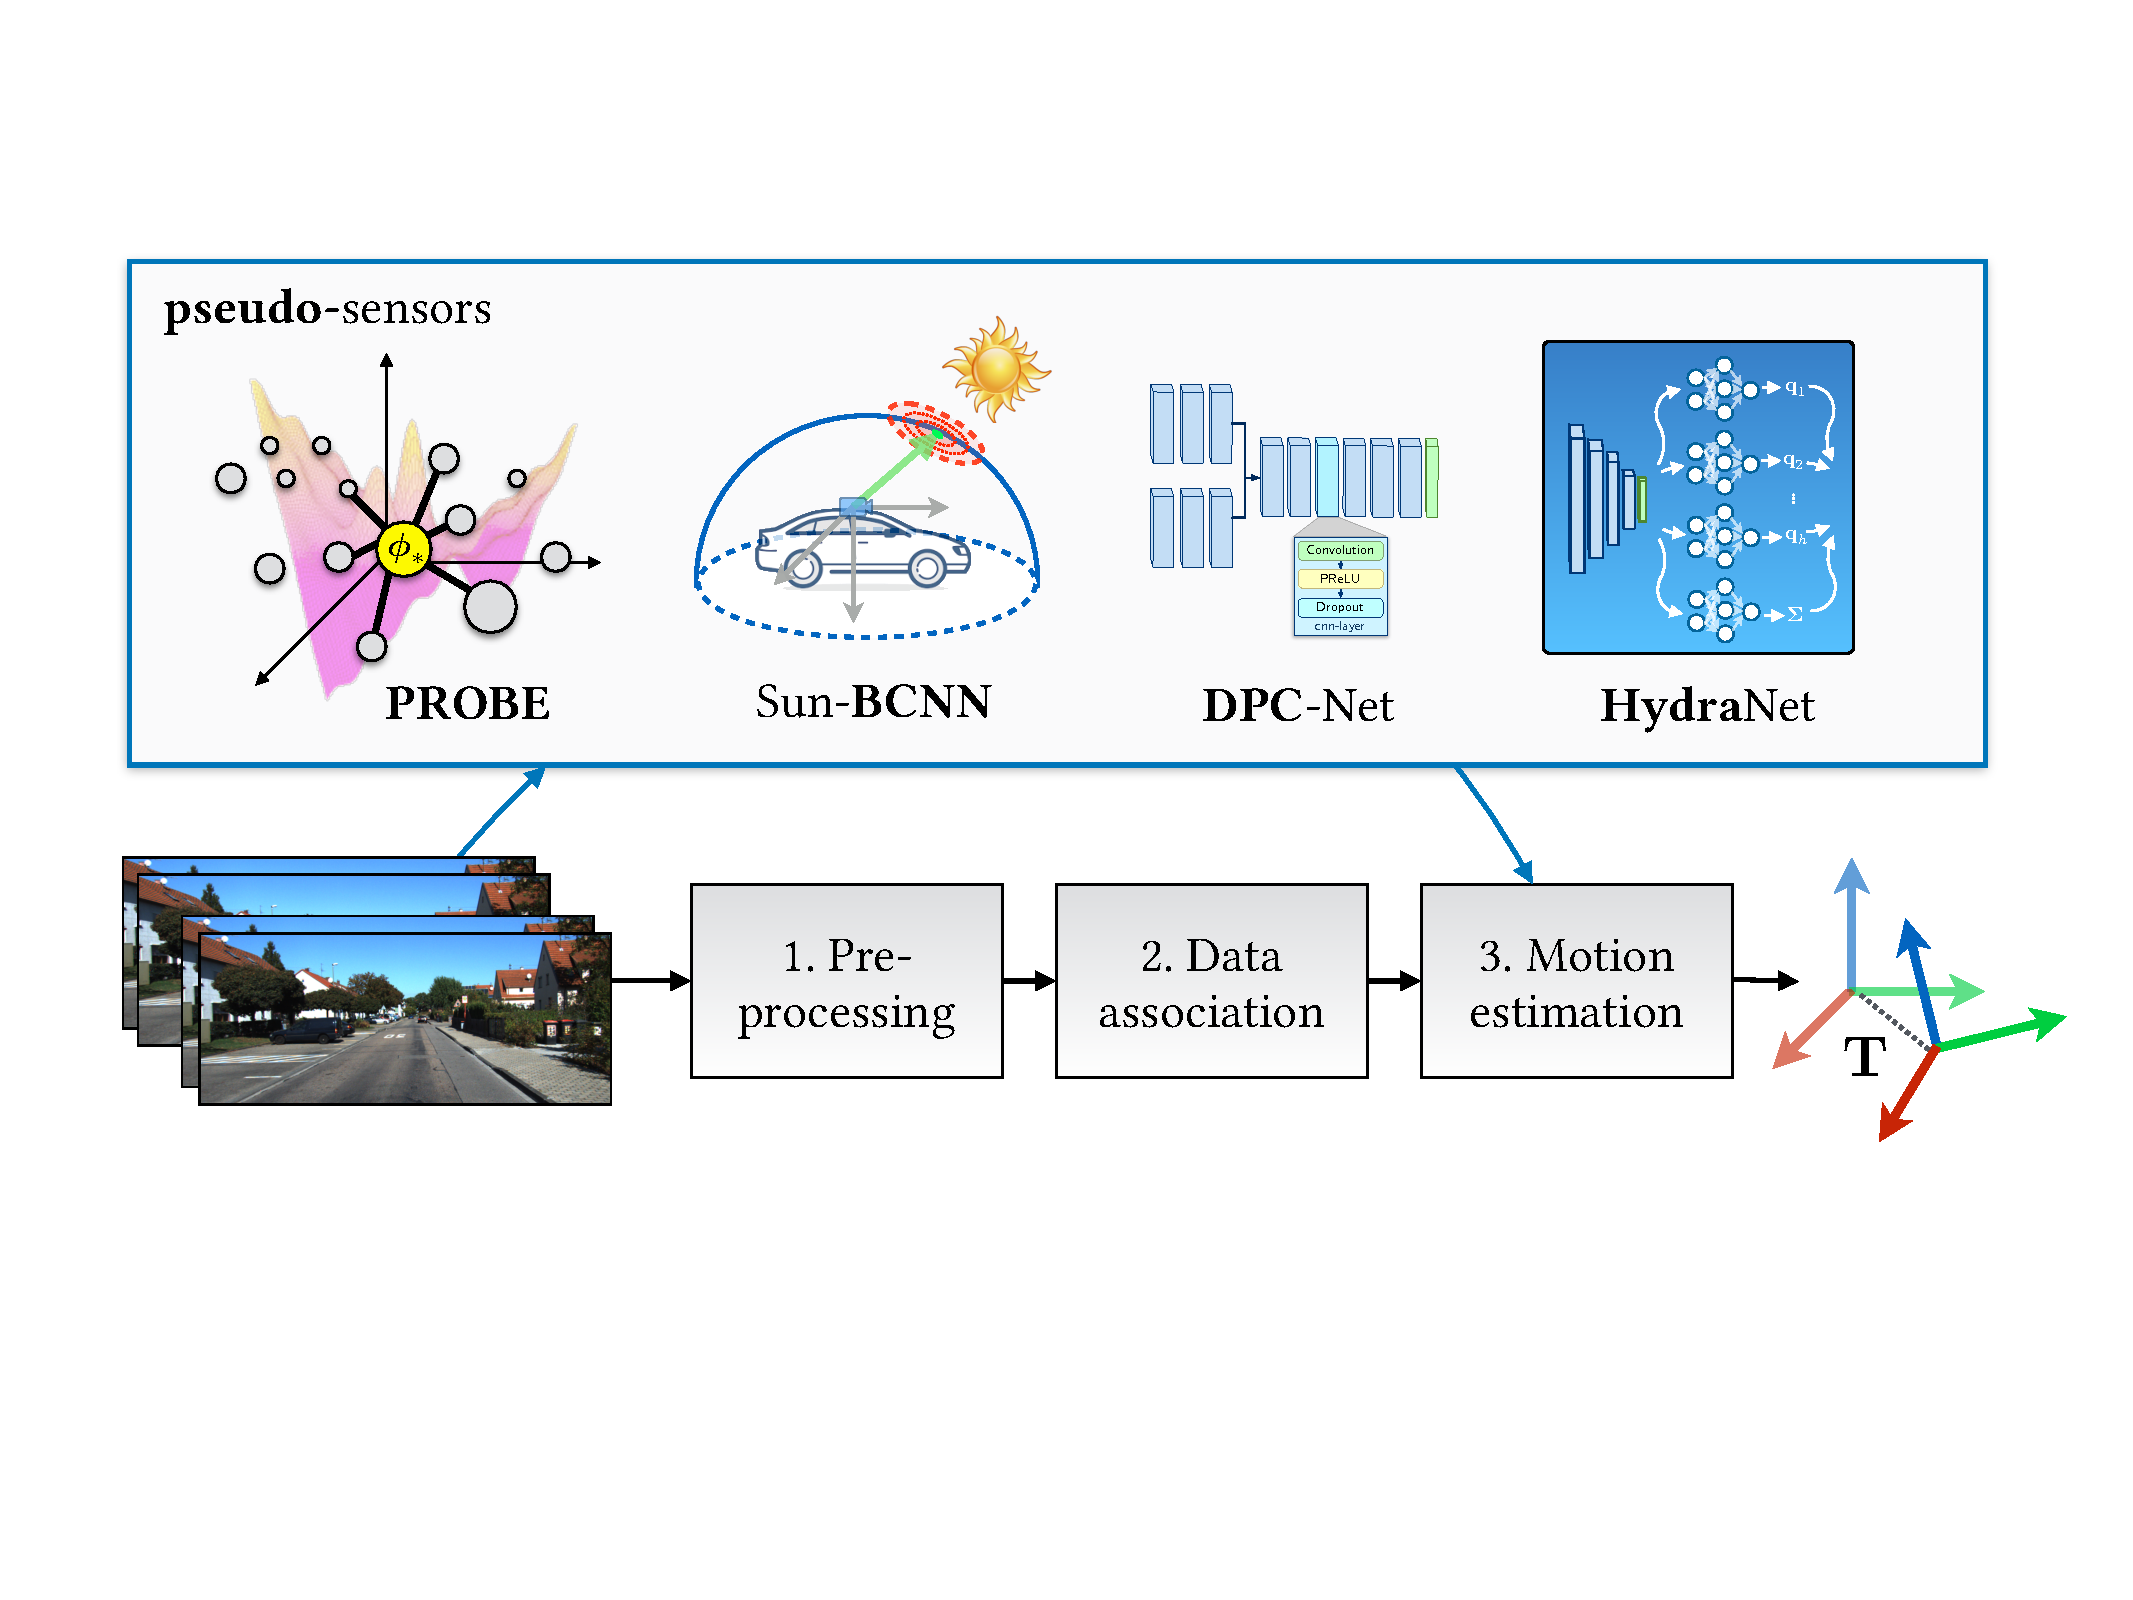
\includegraphics[width=0.98\textwidth]{introduction/all_pseudo_sensors.pdf}
		\caption{My thesis presents four different types of pseudo-sensors to improve visual odometry: PROBE, Sun-BCNN, DPC-Net, and HydraNet.}
  	\label{fig:intro_pseudo_sensors}
\end{center}
\end{figure}


\subsection{Publications}

\begin{enumerate}
\item \textbf{Predictive Robust Estimation for Sparse Visual Odometry} \\
Predictive Robust Estimation (PROBE) is a technique that uses k-NN regression (original PROBE) or Generalized Kernels \citep{Vega-Brown2014-sb} (PROBE-GK) to train a predictive model for heteroscedastic measurement covariance to improve estimator accuracy and consistency.
\begin{itemize}
\item \bibentry{2015_Peretroukhin_PROBE}
\item \bibentry{Peretroukhin2016-om}
\end{itemize}

\item \textbf{Virtual Sun Sensor using a Bayesian Convolutional Neural Network} \\ 
Sun-BCNN is a technique to infer a probabilistic estimate of the direction of the sun from a single RGB image using a Bayesian Convolutional Neural Networks (BCNN). The method works much like dedicated sun sensors \citep{Lambert2012-sn}, but requires no additional hardware, and can provide mean and covariance estimates that can be readily incorporated into existing visual odometry frameworks. I worked on this project in collaboration with Lee Clement. While he focussed on integrating Sun-BCNN into the visual estimator, I developed the BCNN architecture and focused on uncertainty modelling. Initial exploratory work was published at ISER 2016, and the BCNN improvement was presented at ICRA 2017. An additional journal paper summarizing the work of the prior two papers, adding data from the Canadian High Arctic and Oxford, and investigating the effect of cloud cover and transfer learning was published in the International Journal of Robotics' Research, Special Issue on Experimental Robotics at the end of 2017.
\begin{itemize}
\item \bibentry{2017_Clement_Improving}
\item \bibentry{2017_Peretroukhin_Reducing}
\item \bibentry{2018_Peretroukhin_Inferring}
\end{itemize}

\item \textbf{Deep Pose Corrections (DPC-Net)} \\
Deep Pose Correction is a novel approach to improving egomotion estimates through pose corrections learned through deep regression. DPC takes as its starting point an efficient, classical localization algorithm that computes high-rate pose estimates. To it, it adds a Deep Pose Correction Network (DPC-Net) that learns low-rate, `small' \textit{corrections} from training data that are then fused with the original estimates. DPC-Net does not require any modification to an existing localization pipeline, and can learn to correct multi-faceted errors from estimator bias, sensor mis-calibration or environmental effects. 
\begin{itemize}
\item \bibentry{2018_Peretroukhin_Deep}
\end{itemize}

\item \textbf{Probabilistic Inference of Elements of SO(3)}
\begin{itemize}
\item \bibentry{2018_Peretroukhin_Inferring}
\end{itemize}

\end{enumerate}

\subsection{Software Contributions}

\begin{itemize}
\item DPC-Net
\item SO(3) Learning
\item \texttt{liegroups}
\item pyslam 	
\end{itemize}






